\documentclass[twocolumn,11pt,a4paper]{article}
\usepackage[utf8]{inputenc}
\usepackage{mathptmx}
\usepackage[T1]{fontenc}
\usepackage{microtype}
\usepackage{amsmath,amssymb}

%
% DO NOT CHANGE THE FOLLOWING PART
%
\setlength{\textwidth}{6.9in}
\setlength{\textheight}{9.5in}
\setlength{\oddsidemargin}{-0.25in}
\setlength{\evensidemargin}{-0pt}
\setlength{\topmargin}{-0.25in}
\setlength{\columnsep}{0.4in}
\setlength{\parindent}{4ex}
%
\newtheorem{definition}{Definition}
\newtheorem{remark}[definition]{Remark}
\newtheorem{lemma}[definition]{Lemma}
\newtheorem{theorem}[definition]{Theorem}
\newtheorem{proposition}[definition]{Proposition}
\newtheorem{corollary}[definition]{Corollary}
%
%
% THIS IS THE PLACE FOR YOUR OWN DEFINITIONS
%
\newcommand{\R}{\mathbb{R}} % the set of real numbers
%
\DeclareMathOperator*{\nex}{next}
\DeclareMathOperator*{\prev}{prev}
\newcommand{\acro}[1]{\textsc{\lowercase{#1}}}


\usepackage{tikz,pgfplots}
\usetikzlibrary{dateplot}
\usetikzlibrary{shapes,arrows,positioning}
%\usetikzlibrary{dateplot}  
%\usetikzlibrary{pgfplots.groupplots}






% \pgfplotsset{
%    rrbtimeseries/.style={
%         % date coordinates in=x,
%         ylabel=Temperature (K),
%         % legend style={font=\footnotesize},
%         % tick label style={font=\footnotesize},
%         % every axis x label/.style={
%         %   at={(1.3,0)},
%         %   anchor=north,
%         %   },
%         % label style={font=\footnotesize},
%         % xticklabel style= {rotate=17,anchor=north east},
% %        every axis title shift=0pt,
% %        max space between ticks=15,
%        %  every mark/.append style={mark size=6},
%        %  major tick length=0.1cm,
%        %  minor tick length=0.066cm,
%        %  very thin,
%        %  every axis legend/.append style={
%        %    at={(1.2,0)},
%        %    anchor=south east,
%        %    draw = none},
%        % legend columns = 4,
%        % unbounded coords=jump, %v>1.4
%     },

%   % rrbrs/.style={
%   %       rrbtimeseries,
%   %       width = \textwidth,
%   %       height = 0.25\textwidth,
%   %       every axis x label/.style={
%   %         at={(1.3,-1)},
%   %         anchor=north,
%   %         },
%   %       ylabel = {},  
%   %       max space between ticks=50,
%   %       every axis legend/.append style={
%   %         at={(1,-1.1)},
%   %         anchor=north east,
%   %         draw = none},
%   %       title style={font=\small,below,anchor=north,fill=white},
%   %   },
%  }




\pgfplotsset{
   timeseries/.style={
        date coordinates in=x,
        ylabel=Temperature (K),
        legend style={font=\footnotesize},
        tick label style={font=\footnotesize},
        every axis x label/.style={
          at={(1.3,0)},
          anchor=north,
          },
        label style={font=\footnotesize},
        xticklabel style= {rotate=17,anchor=north east},
%        every axis title shift=0pt,
%        max space between ticks=15,
        every mark/.append style={mark size=6},
        major tick length=0.1cm,
        minor tick length=0.066cm,
        very thin,
        every axis legend/.append style={
          at={(1.2,0)},
          anchor=south east,
          draw = none},
       legend columns = 4,
    },
    rd/.style={
        timeseries,
        every axis x label/.style={
          at={(1.3,-1)},
          anchor=north,
          },
        label style={font=\footnotesize},
        ylabel = {},
        width=17cm,
        height=3.5cm,   
        max space between ticks=50,
        every axis legend/.append style={
          at={(1,-1.1)},
          anchor=north east,
          draw = none},
        title style={font=\small,below, at={(0.7,1.7)},anchor=north,fill=white},
    }
}


%        unbounded coords=jump, %v>1.4
%        unbounded coords=discard, %v>1.4


%http://tex.stackexchange.com/questions/46422/axis-break-in-pgfplots

%http://tex.stackexchange.com/questions/52409/insert-a-separate-mark-inside-a-pgfplots-graph

\usepackage[
style=numeric-comp,
sortcites=true,
% backref=true,
]{biblatex}
\bibliography{bibliografia}
\ExecuteBibliographyOptions{
  isbn=false,url=false,doi=false,eprint=false,alldates=terse,firstinits=true,abbreviate=true,maxnames=2,
}
\bibitemsep 0mm \bibnamesep 0mm \bibinitsep 0mm \biblabelsep 1mm \bibhang 0mm 


\renewcommand*\newunitpunct{\addcomma\addspace}
\DeclareFieldFormat[inproceedings]{booktitle}{}
\DeclareFieldFormat{volume}{}
\DeclareFieldFormat[inproceedings]{title}{#1}
\DeclareFieldFormat[book]{title}{#1}
\DeclareFieldFormat[article]{title}{#1}
\DeclareFieldFormat[incollection]{title}{#1}
\DeclareFieldFormat[collection]{title}{#1}
\DeclareFieldFormat[online]{title}{#1}

\DeclareFieldFormat{series}{\em #1}
\DeclareFieldFormat{pages}{\small pp#1}

\renewbibmacro*{title}{%
  \printfield{title}
}

\renewbibmacro*{publisher+location+date}{%
  \printlist{publisher}%
  \newunit
  \printfield{year}%
  \newunit
}

\renewbibmacro*{issue+date}{%
  \newunit
  \printfield{year}
}

\renewbibmacro*{in:}{
}

\newbibmacro*{in:collection}{
  \printtext{%
    \bibstring{in} \cite{\thefield{crossref}}}
%  \newunit
%  \cite{\thefield{crossref}}
}

%http://www.tex.ac.uk/tex-archive/macros/latex/contrib/biblatex/latex/

\DeclareBibliographyDriver{incollection}{%
  \usebibmacro{bibindex}%
  \usebibmacro{begentry}%
  \usebibmacro{author/translator+others}%
  \setunit{\labelnamepunct}\newblock
  \usebibmacro{title}%
  \newunit
  \printlist{language}%
  \newunit\newblock
  \usebibmacro{byauthor}%
  \newunit\newblock
%  \usebibmacro{in:}%
  \usebibmacro{in:collection}%
%  \usebibmacro{maintitle+booktitle}%
%  \newunit\newblock
%  \usebibmacro{byeditor+others}%
%  \newunit\newblock
%  \printfield{edition}%
%  \newunit
%  \iffieldundef{maintitle}
%    {\printfield{volume}%
%     \printfield{part}}
%    {}%
%  \newunit
%  \printfield{volumes}%
%  \newunit\newblock
%  \usebibmacro{series+number}%
%  \newunit\newblock
%  \printfield{note}%
%  \newunit\newblock
%  \usebibmacro{publisher+location+date}%
  \newunit\newblock
  \usebibmacro{chapter+pages}%
%  \newunit\newblock
%  \iftoggle{bbx:isbn}
%    {\printfield{isbn}}
%    {}%
%  \newunit\newblock
%  \usebibmacro{doi+eprint+url}%
%  \newunit\newblock
%  \usebibmacro{addendum+pubstate}%
  \setunit{\bibpagerefpunct}\newblock
  \usebibmacro{pageref}%
  \newunit\newblock
%  \usebibmacro{related}%
  \usebibmacro{finentry}}


%a cada secció hi ha un vspace
\makeatletter

\let\old@section\section

\renewcommand*{\section}{%
  \@ifstar{%
    \starsection
  }{%
    \@dblarg\nostarsection
  }%
}
\newcommand*{\starsection}[1]{%
  \vspace{-12pt}
  \old@section*{#1}%
  \vspace{-10pt}%
}
\newcommand{\nostarsection}{}
\def\nostarsection[#1]#2{%
  % #1: toc entry
  % #2: main entry
  \vspace{-7pt}
  \old@section[{#1}]{#2}%
  \vspace{-6pt}%
}

\let\old@subsection\subsection
\renewcommand\subsection[2][]{\vspace{-11pt}\old@subsection[#1]{#2}\vspace{-7pt}}

\let\old@mathbb\mathbb
\renewcommand\mathbb[2][]{{\rm I}\!{\rm #2}}

\makeatother

% redimensió de les llistes
\usepackage{enumitem}
\setitemize{topsep=1pt,itemsep=1pt,leftmargin=8pt,labelwidth=6pt}


%espai caption figures
\setlength{\abovecaptionskip}{0cm}

%
%
% THE BEGINNING OF THE DOCUMENT
%
\begin{document}
\global\def\refname{{\normalsize \it References:}}
%
\baselineskip 12.5pt
%
%
% TITLE, AUTHOR, ABSTRACT, KEYWORDS
%
\title{\LARGE \bf A Model for a Multiresolution Time Series Database
  System}

\date{}

\author{\hspace*{-10pt}
  \begin{minipage}[t]{2.3in} \normalsize \baselineskip 12.5pt
    \centerline{\scshape A.~LLUSÀ-SERRA}
  \end{minipage} \kern 0in
  \begin{minipage}[t]{2.3in} \normalsize \baselineskip 12.5pt
    \centerline{\scshape T.~ESCOBET-CANAL}
  \end{minipage} \kern 0in
  \begin{minipage}[t]{2.3in} \normalsize \baselineskip 12.5pt
    \centerline{\scshape S.~VILA-MARTA}
  \end{minipage} \\ \hspace*{-10pt}
  % 
  \begin{minipage}[t]{2.7in} \normalsize \baselineskip 12.5pt
    \centerline{Universitat Politècnica de Catalunya}
    \centerline{Department of Electronic Systems Design and Programming}
    \centerline{Av.~Bases de Manresa 61--73, 08242 Manresa}
    \centerline{\scshape ES-CT}
  \end{minipage}
  \\[14pt]
  \begin{minipage}[t]{2.3in} \normalsize \baselineskip 12.5pt
    \centerline{aleix@dipse.upc.edu}
  \end{minipage} \kern 0in
  \begin{minipage}[t]{2.3in} \normalsize \baselineskip 12.5pt
    \centerline{teresa.escobet@upc.edu}
  \end{minipage} \kern 0in
  \begin{minipage}[t]{2.3in} \normalsize \baselineskip 12.5pt
    \centerline{sebas@dipse.upc.edu}
  \end{minipage} 
  % % 
  % If you are three authors then you can use three mini--pages
  % instead of two. Their horizontal size must be less than 2.7in
  % indicated above. It can be e.g. 2.3in. However, you must pay
  % attention that you do not exceed the total width of the text.
  % 
  \\[5pt]
  \begin{minipage}[b]{6.9in} \normalsize
    \baselineskip 12.5pt {\it Abstract:}
    % The text of the abstract follows.
    In this paper we propose a model for multiresolution time series
    database management systems. This model stores compactly a time series
    and manages consistently its temporal dimension. This is achieved by
    extracting different resolutions and attributes summaries from the
    original time series.
    % 
    Our work is concerned in putting together two areas of study: time
    series analysis and database management systems. Time series analysis
    offers a great deal of methodologies and algorithms to process time
    series data. Database systems field provides software expertise in
    managing data. Therefore, for many applications it is of primary
    relevance that database systems support time series.
    % 
    \\[4mm] \textit{Key--Words:}
    % The key-words follow.
    time series, data model, database systems, monitoring systems.
  \end{minipage}
  \vspace{-10pt}
}

\maketitle

\thispagestyle{empty} \pagestyle{empty}
% numbers of pages are supplemented by the editor
%
% THE BEGINNING OF THE TEXT
%

%intro, requirements
\section{Introduction}

% Modern society depends on the expert operation of many complex
% engineering systems which provides products and services. Examples
% include electric power systems, water distributions networks,
% transportation systems, manufacturing processes, intelligent
% buildings, communication systems, etc. The emergence of embedded
% systems and sensor networks has made possible the collection of large
% amounts of data for monitoring and control of such complex systems. In
% most application, these data need to be processed and synthesised
% efficiently to provide relevant information to engineers, researchers,
% accident investigators, operators, and many other users.

The emergence of embedded systems and sensor networks has made
possible the collection of large amounts of data for monitoring and
control of complex systems.
%
Nevertheless, before using the collected signals, it is of primary
importance to detect the eventual sensor failures or malfunctions and
to reconstruct the incorrect signals. This avoids to process
misleading information which may lead to unsafe or inefficient
actions. Acquired data is associated with a time stamp, which implies
that the correctness of those data depends not only on the measured
value but also on the time as it is collected. When observations are
collected at specific time intervals, large data sets in the form of
time series are generated, \cite{basu07:_autom}.

Time series are defined as a collection of observations made
chronologically, \cite{fu11}, accordingly they are also called time
sequences \cite{last:hetland}.  Time series are usually stored in a
database. Usually the managing software to store this data are
relational database management systems (RDBMS). However, using a RDBMS
as a time series backend suffers some drawbacks,
\cite{dreyer94,schmidt95,stonebraker09:scidb,zhang11}. Time series
come from a continuous nature in which they are recorded at regular
intervals, such as hourly or daily, or at irregular intervals, such as
recording when a pump is open or closed.

There are two main problems when managing time series. The first
results from these data being voluminous, \cite{fu11}. Because of
this, storing and accessing them can be difficult. Moreover, this is
critical when developing small embedded systems, whose resources
(capacity, energy, processing, and communications) suffer a genuine
restriction, \cite{yaogehrke02}.  The second problem concerns the
procedure of processing and synthesising information from the time
series data, that becomes challenging when data is not equi-time
spaced.



%TSMS

This paper focuses on Data Base Management Systems (DBMS) that store
and treat data as time series. These are usually known as Time Series
Data Base Management Systems (TSMS), \cite{dreyer94}.  We introduce a
new data model for a multiresolution TSMS (MTSMS). This model allows
to store time series using different time resolutions and it organizes
data in an aggregated way. It is designed to cope well with bounded
storage computers such as sensor systems.

The paper is organised as follows.  In Section~\ref{sec:related-work}
some related work concerning TSMS are presented and a summary of its
features is shown in Section~\ref{sec:tsms-features}.  The MTSMS model
is formalized as follows: the nomenclature preliminaries are
introduced in Section~\ref{sec:model:preliminaries}, the data
structure is formulated in Section~\ref{sec:MTSMS}, and attribute
aggregation is summarised in
Section~\ref{sec:model:interpolador}. Section~\ref{sec:example} is
devoted to a real data multiresolution database example. Finally,
Section~\ref{sec:concl-future-work} offers final
conclusions.% and we consider some future working directions.



\section{Related work}
\label{sec:related-work}

There are some prior works concerning TSMS. 
%
RRDtool from Oetiker, \cite{rrdtool}, is a free software database
management system. It is designed to be used for monitoring
systems. Because of this, it is focused to a particular kind of data,
gauges and counters, and it lacks general time series
operations. RRDtool can store multiple time resolution data. The work
in this paper is partially inspired in RRDtool.

Cougar, \cite{bonnet01}, is a sensor database system. It has two main
structures: one for sensor properties stored into relational tables
and another for time series stored into data sequences from
sensors. Time series have specific operations and can combine
relations and sequences. Cougar target field is sensor networks, where
data is stored distributed in sensors. Queries are resolved combining
sensor data in a data stream orientation, which improves processing
performance.
% However, data streams imposes restriction on
% operators so this TSMS can not be generalised to other time series
% types. 
%% Moreover, sequences and relations can collide in representing ambiguously time series.

SciDB, \cite{stonebraker09:scidb}, and SciQL, \cite{zhang11}, are
array database systems. These systems are intended for science
applications, in which time series play a principal role. They
structure time series into arrays in order to achieve multidimensional
analysis and allow tables to store other data.  Although SciDB is
based on arrays which, according to the authors, include time series,
it does not consider time series special needs: it does not considers
how to manage continuously voluminous data neither how to achieve
temporal coherence.  In contrast, SciQL exhibits some time series
managing chraracteristics that include time series regularities,
interpolation or correlation queries.  However, difference between
tables and arrays seems too physical and leads to ambiguously
representing time series.

Bitemporal DBMS is another database field related with
time. Bitemporal data target is to keep historical events in the
database by associating time intervals to data.  Bitemporal data and
time series data are not exactly the same and so can not be treated
interchangeably, \cite{schmidt95}. However, there are some
similarities %between time series and bitemporal data
that can be considered. First, extending a relational model to manage
bitemporal data illustrate the extension of RDMBS with new types and
how to model them. Second, bitemporal data modelling settles some
time-related concepts that can be extended to time series.

The recent bitemporal data research in relational DBMS model terms,
\cite{date02:_tempor_data_relat_model}, marks a promising
foundation. It models bitemporal data as relations extended with time
intervals attributes and extends relational operations in order to
deal with related time aspects.





\section{TSMS features}
\label{sec:tsms-features}

A TSMS is a special purpose DBMS aimed at storing and managing time
series. The main objective of TSMS is to put together two areas of
study: time series analysis and DBMS.  Time series analysis formalises
a great amount of algorithms and methodologies that apply to time
series, with a main focus on improving efficiency. DBMS theory
formalises systems that store and operate with data; currently the
relation model \cite{date:introduction} is the referent.

In time series analysis there are some common operations that can be
generalised when managing time series.
%
The main attribute of time series is the time, therefore dealing with
time is a common operation, such as querying time intervals, finding
time correlations, or calculating distances between two time
series. TSMS must respect the temporal coherence of the time series.
In the context of statistics, aggregation of time series is also
common operation. Aggregation consists in summarising a time series
subset with an attribute such as the mean, the maximum, or the mode.

A particular feature of time series is representation. A time series
is discrete in the set sense, that is a set of value and time
pairs. Representation is the function model approximating the time
series to its continuous nature. TSMS operate on time series
respecting the representation coherence. Furthermore, the values of a
time series can be of any type.
% , preferably using piecewise operations in the set domain rather
% than solving numerical methods for the continuous domain.





%MTSMS
%\subsection{Multiresolution features}
%\subsection{Multiresolution motivation example}

A MTSMS is a TSMS with multiresolution capabilities.
In a MTSMS a schema has to be configured, which mainly consist in
defining different pairs of a time resolution and an attribute summarising
function. 
%We show it with an example.

% Figures \ref{fig:mtsms:sequence} and
% \ref{fig:mtsms:sequence-irregular} show a multiresolution summary for
% a regular and irregular time series, respectively. Both figures show a
% snapshot in time, suppose between time 9 and 10.


% \begin{figure}[tp]
%   \centering
%   %\usetikzlibrary{positioning}
\begin{tikzpicture}[scale=0.77, every node/.style={transform shape}]

  %referencia
  \node (-6) {};

  \foreach \x in {-5,...,12}
  {
    \pgfkeys{/pgf/number format/.cd,int trunc}
    \pgfmathparse{abs(\x)}
    \let\absx=\pgfmathresult
    \pgfmathparse{\x-1}
    \let\antx=\pgfmathresult
    %time
    \node[node distance=1mm] (\x) [right=of \antx] 
    {\ifnum\x<11 \x \else \phantom{9} \fi};

    %graph values
    \node [above=\absx mm of \x] 
    {\ifnum\x=10 \color{gray} \fi \ifnum\x<11 $\bullet$ \fi};    

    %values
    % \node[rectangle,draw] (s\x) [below=of \x] 
    % {\ifnum\x<10 \pgfmathprintnumber{\absx} \else \phantom{9} \fi};
    \ifnum\x<10
    \node[rectangle,draw] (s\x) [below=of \x] 
    {\pgfmathprintnumber{\absx}};
    \else
    \node[rectangle,dotted,draw] (s\x) [below=of \x] 
    {\phantom{9}};
    \fi
  }

  \node [below=of 10] {\color{gray}10}; 
  

  
  %rd: 5s |inf| mean
  \node [circle,draw] (rd5-5) [below=3cm of s-5] {u};
  \node [circle,draw] (rd50) [below=3cm of s0] {u};
  \node [circle,draw] (rd55) [below=3cm of s5] {3};
  \node [circle,dotted,draw] (rd510) [below=3cm of s10] {\color{gray}u};
  \node [below=3.3cm of s10] {\color{gray}8};
 
  \draw[->,bend right] (s5) to (rd55);
  \draw[->,bend right] (s4) to (rd55);
  \draw[->,bend right] (s3) to (rd55);
  \draw[->,bend right] (s2) to (rd55);
  \draw[->,bend right] (s1) to (rd55);

  \draw[->,dotted,bend right] (s10) to (rd510);
  \draw[->,bend right] (s9) to (rd510);
  \draw[->,bend right] (s8) to (rd510);
  \draw[->,bend right] (s7) to (rd510);
  \draw[->,bend right] (s6) to (rd510);

  
  %rd: 3s |inf| mean
  \node [circle,draw] (rd3-3) [below=of s-3] {u};
  \node [circle,draw] (rd30) [below=of s0] {u};
  \node [circle,draw,fill=white] (rd33) [below=of s3] {2};
  \node [circle,draw,fill=white] (rd36) [below=of s6] {5};
  \node [circle,draw,fill=white] (rd39) [below=of s9] {8};
  \node [circle,dotted,draw] (rd312) [below=of s12] {\color{gray}u};

  \draw[->] (s3) to (rd33);
  \draw[->] (s2) to (rd33);
  \draw[->] (s1) to (rd33);

  \draw[->] (s6) to (rd36);
  \draw[->] (s5) to (rd36);
  \draw[->] (s4) to (rd36);

  \draw[->] (s9) to (rd39);
  \draw[->] (s8) to (rd39);
  \draw[->] (s7) to (rd39);

  \draw[->,dotted] (s12) to (rd312);
  \draw[->,dotted] (s11) to (rd312);
  \draw[->,dotted] (s10) to (rd312);



  %eixos
  \node (et0) [above=1mm of -5] {};
  \node (et12) [above=1mm of 11] {};
  \node [right=-2mm of et12] {time};
  \draw[->] (et0) to (et12);
  \node (y5) [above=5mm of 0] {--};
  \node [left=-1.5mm of y5] {5};
  \node (y10) [above=10mm of 0] {--};
  \node [left=-1.5mm of y10] {10};

  \node (inici) [above=4cm of s0] {init};
  \node (inici2) [below=4cm of s0] {};
  \draw[-,dotted] (inici) to (inici2);

  \node (fi) [above=4.4cm of s9.east] {now};
  \node (fi2) [below=4.4cm of s9.east] {};
  \draw[-,dotted] (fi) to (fi2);


  \node (fut) [below right=1mm and 1mm of fi] {future};
  \draw[->] (fut.south west) to (fut.south east);

  \node (pas) [below left=1mm and 1mm of fi] {past};
  \draw[->] (pas.south east) to (pas.south west);

  \node (unk) [below left=1mm and 1mm of inici] {unknown};
  \draw[->] (unk.south east) to (unk.south west);



  \node [above=0cm of s-5] {\makebox[0cm][l]{sample every 1 u.t.}};
  \node [below=0.5cm of s-5] {\makebox[0cm][l]{mean every 3 u.t.}};
  \node [below=2.5cm of s-5] {\makebox[0cm][l]{mean every 5 u.t.}};


\end{tikzpicture}



%%% Local Variables:
%%% TeX-master: "../main"
%%% ispell-local-dictionary: "british"
%%% End:

%   \caption{Multiresolution snapshot diagram with regular sampling}
%   \label{fig:mtsms:sequence}
% \end{figure}


% \begin{figure}[tp]
%   \centering
%   %\usetikzlibrary{positioning}
\begin{tikzpicture}

  \node[node distance=1mm] (0) {0};
  \node[node distance=1mm] (-1) [left=of 0]{\phantom{9}};
  \node[node distance=1mm] (1) [right=of 0] {\phantom{1}};
  \node[node distance=1mm] (2) [right=of 1] {2};
  \node[node distance=1mm] (3) [right=of 2] {\phantom{3}};
  \node[node distance=1mm] (4) [right=of 3] {4};
  \node[node distance=1mm] (5) [right=of 4] {\phantom{5}};
  \node[node distance=1mm] (6) [right=of 5] {6};
  \node[node distance=1mm] (7) [right=of 6] {\phantom{7}};
  \node[node distance=1mm] (8) [right=of 7] {8};
  \node[node distance=1mm] (9) [right=of 8] {\phantom{9}};
  \node[node distance=1mm] (10) [right=of 9] {10};
  \node[node distance=1mm] (11) [right=of 10] {\phantom{9}};
  \node[node distance=1mm] (12) [right=of 11] {\phantom{9}};


  \node [above=0 mm of 0] {$\bullet$}; 
  \node [above=2 mm of 2] (v2) {$\bullet$}; 
  \node [above=4 mm of 4] {?}; 
  \node [above=6 mm of 6] (v6) {$\bullet$}; 
  \node [above=7 mm of 7] {$\bullet$}; 
  \node [above=9 mm of 9] {$\bullet$}; 
  \node [above=10 mm of 10] (v10) {$\bullet$}; 


  \node[rectangle,draw] (s0) [below=of 0] {0};
  \node[rectangle,draw] (s2) [below=of 2] {2};
  \node[rectangle,draw] (s4) [below=of 4] {u};
  \node[rectangle,draw] (s6) [below=of 6] {6};
  \node[rectangle,draw] (s7) [below=of 7] {7};
  \node[rectangle,draw] (s9) [below=of 9] {9};
  \node[rectangle,draw] (s10) [below=of 10] {\color{gray}10};
  \node[rectangle,draw] (s11) [below=of 11] {\phantom{9}};
  \node[rectangle,draw] (s12) [below=of 12] {\phantom{9}};


  \draw[<->] (v2.north east) to (v6.north west)
  node [above,sloped,midway] {\small gap};

  \draw[<->] (v6.south east) to (v10.south west)
  node [below,sloped,midway] {\small irregular};

  
  %rd: 5s |inf| mean
  \node [circle,draw] (rd50) [below=4cm of 0] {u};
  \node [circle,draw] (rd55) [below=4cm of 5] {2};
  \node [circle,draw] (rd510) [below=4cm of 10] {u};
  \node [below=4.3cm of 10] {\color{gray}8};
 
  \draw[->,bend right] (s4) to (rd55);
  \draw[->,bend right] (s2) to (rd55);

  \draw[->,dotted,bend right] (s10) to (rd510);
  \draw[->,bend right] (s9) to (rd510);
  \draw[->,bend right] (s7) to (rd510);
  \draw[->,bend right] (s6) to (rd510);

  
  %rd: 3s |inf| mean
  \node [circle,draw] (rd30) [below=of s0] {u};
  \node [circle,draw,fill=white] (rd33) [below=2.5cm of 3] {2};
  \node [circle,draw,fill=white] (rd36) [below=2.5cm of 6] {5};
  \node [circle,draw,fill=white] (rd39) [below=2.5cm of 9] {8};
  \node [circle,draw] (rd312) [below=2.5cm of 12] {u};

  \draw[->] (s2) to (rd33);

  \draw[->] (s6) to (rd36);
  \draw[->] (s4) to (rd36);

  \draw[->] (s9) to (rd39);
  \draw[->] (s7) to (rd39);

  \draw[->,dotted] (s12) to (rd312);
  \draw[->,dotted] (s11) to (rd312);
  \draw[->,dotted] (s10) to (rd312);



  %eixos
  \node (et0) [above=1mm of -1] {};
  \node (et12) [above=1mm of 11] {};
  \node [right=-2mm of et12] {time};
  \draw[->] (et0) to (et12);
  \node (y5) [above=5mm of 0] {--};
  \node [left=-1.5mm of y5] {5};
  \node (y10) [above=10mm of 0] {--};
  \node [left=-1.5mm of y10] {10};

  \node (inici) [above=3.1cm of s0] {init};
  \node (inici2) [below=3.3cm of s0] {};
  \draw[-,dotted] (inici) to (inici2);

  \node (fi) [above=3.4cm of s9.east] {now};
  \node (fi2) [below=3.5cm of s9.east] {};
  \draw[-,dotted] (fi) to (fi2);


  % \node (fut) [below right=1mm and 1mm of fi] {future};
  % \draw[->] (fut.south west) to (fut.south east);

  % \node (pas) [below left=1mm and 1mm of fi] {past};
  % \draw[->] (pas.south east) to (pas.south west);

  \node [above=0cm of s0] {\makebox[0.5cm][l]{sample every 2 u.t.}};
  \node [below=0.5cm of s0] {\makebox[0.5cm][l]{mean/3}};
  \node [below=2cm of s0] {\makebox[0.5cm][l]{mean/5}};

\end{tikzpicture}



%%% Local Variables:
%%% TeX-master: "../main"
%%% ispell-local-dictionary: "british"
%%% End:

%   \caption{Multiresolution snapshot diagram with irregular sampling}
%   \label{fig:mtsms:sequence-irregular}
% \end{figure}

% At the top of the figures there is a plot of a time series with time
% axis in general units of time (u.t.) and with value axis in
% undetermined units. The 'now' point shows when the snapshot has been
% taken, so the time before is the past and the time after is the
% future, which is grey coloured. The 'init' point shows when the
% database system has started sampling, so data in time before is
% unknown; we indicate the starting point as being zero u.t.\ and unknown
% time points with negative units.

% At the bottom of the figures there is a digram showing the
% multiresolution action. The first row shows the numerical time series'
% values corresponding to the above plot; in
% fig.~\ref{fig:mtsms:sequence} the time series is sampled every one
% unit of time and in fig.~\ref{fig:mtsms:sequence-irregular} every
% two. The second and the third row show a particular schema of a
% multiresolution database consisting in two time resolutions for the
% time series: one computes the mean of the sampled values every three
% u.t.\ and the other computes the mean every five u.t. In this example,
% computing the mean acts as the attribute summarising function of which
% we have spoken earlier. All data stored before zero time, this
% included, is unknown as sampling had not started. For the future
% values we also simulate as having unknown stored values which will
% change as time advances.

% If we look at fig.~\ref{fig:mtsms:sequence} we see, drawn by arrows,
% that every three sampled values a mean is stored and independently
% every five values another mean is stored. For the future values we
% show in gray that if we advance the time one u.t.\ then value 10 is
% sampled an the mean for time 10 can be computed resulting 8 but not
% yet the mean for time 12.

% Fig.~\ref{fig:mtsms:sequence-irregular} is essentially the same but
% showing two possible monitoring irregularities: a gap and a time
% disruption. In other words, we want to sample the time series every 2
% u.t.\ but first for some reason it can not be done in time 4 and
% second the sampling clock is disrupted and samples are done in time 7
% and 9 instead of 8. The resulting stored time schema is the same: on
% time resolution every 3 u.t.\ and the other every 5 u.t.; that is,
% without time disruptions. The resulting stored values are computed
% from the known sampled values, some coincide with
% fig.~\ref{fig:mtsms:sequence} whereas some differ specially in the
% gap. A better function than mean would solve this, we extend this
% further in section~\ref{sec:model:interpolador}.





% MTSMS improve TSMS features in various aspects:
% \begin{itemize}

% \item Voluminous data. Monitoring systems capture a huge amount of
%   data from sensors. In order to be able to process this information,
%   data volume must be reduced. With the multiresolution approach only
%   the most interesting segments of data are stored. This segments are
%   seen as different resolutions for the same time series and the user
%   configures how they are extracted and summarised by defining
%   different consolidation steps and functions. Multiresolution can
%   also be useful at visualisation time as the user is able to select
%   the best time range and time step that fits into the screen; there
%   is no need to process with more quantity of data than the one that
%   can be shown. In figure~\ref{fig:mtsms:sequence} there is an example of
%   extracting two resolutions: one every three units of time and
%   another every five.

% \item Data validation. Monitoring systems capture data but can occur
%   some drawbacks that will affect later the process of time series
%   analysis. Main problems are found when monitors can not capture
%   data, known as gaps, or capture data erroneously, such as outlayers.
%   The multiresolution attribute functions cope well with validating,
%   filtering and calculating with this unknown data in order to keep a
%   consistent historic. In figure~\ref{fig:mtsms:sequence-irregular} an
%   example of a gap can be seen.

% \item Data time regularising. Another monitoring side effect happens
%   when the sampling rate is not constant, that is when the resulting
%   data is not equi-time spaced. This no regularities can come from
%   sampling jitters in periodic sampling or from no periodic
%   event-based sampling. The multiresolution consolidation regularises
%   the time interval when processes a time series, therefore each
%   resulting time series segment has a regular time resolution. This
%   regularising approach could also be used when the user wants to
%   consult another resolution for a time series, such as changing
%   periodic data from a month to a year step. In
%   figure~\ref{fig:mtsms:sequence-irregular} an example of time
%   regularising can be seen.

% \item Information summaries. Time series analysis typically focuses on
%   reconstructing the original signal. However, the user objective in a
%   database system is to consult some information. The multiresolution
%   approach is a lossy compression storage solution for data. Therefore
%   it can be regarded as not only approximating to the original time
%   series function but also extracting the interesting information. The
%   selected information must be determined a priori assuming the
%   context where the future queries will be done. In
%   figure~\ref{fig:mtsms:sequence} there is an example of summarising by
%   mean attribute.

% \end{itemize}











%%% Local Variables:
%%% TeX-master: "main-wseas"
%%% ispell-local-dictionary: "british"
%%% End:

% LocalWords:  multiresolution TSMS


%model MTSMS
\section{Preliminaries}
\label{sec:model:preliminaries}

In this section we introduce some background concepts and the
nomenclature which we will use later.  First we define the main
objects of a \acro{MTSMS} which are measures and time series.

A \emph{measure} is a value measured in a time instant. More formally
it is a tuple $(v,t)$ where $v$ is the value of the measure and $t \in
\mathbb{R}$ is the time instant of measurement.  The values of a time
series can be of any type. For simplicity examples are presented with
integers or real numbers but can also be strings or vectors.  Let $m =
(v,t)$ be a measure, $v$ is written as $V(m)$ and $t$ is written as
$T(m)$.

The time value defines the canonical order between measures.  Let $m =
(v_m, t_m)$ and $n = (v_n, t_n)$ be two measures, then $m\geq n$ if
and only if $t_m\geq t_n$.

A \emph{time series} is sequence of measures of the same phenomena
that are ordered in time.
\begin{definition}[Time series]
  A \emph{time series} $S$ is a a set of measures of the same
  phenomena $S = \{m_0, \ldots, m_k\}$ without repeated time values
  $\forall i,j: i\leq k, j\leq k, i\neq j : T(m_i)\neq T(m_j)$. Given
  a time series $|S|$, we note its size by $|S|=k+1$. Observe that,
  because measures in $S$ are of the same phenomena, the type of $S$
  values is homogeneous.
\end{definition}

The order defined by measures implies a total order in a time
series. As a time series is a finite set, if it is not empty it has a
maximum and a minimum.  Let $S=\{m_0,\ldots,m_k\}$ be a time series
and $n\in S$ be a measure. The time series' maximum is $n=\max(S)$ if
and only if $\forall m \in S: n \geq m $.  Similarly, the time series'
minimum is $n=\min(S)$ if and only if $\forall m \in S: n \leq m$.

Given the order defined by time, in a time series we define the
sequence interval following \cite{last:keogh,last:hetland}.  Let
$S=\{m_0, \ldots, m_k\}$ be a time series. We define the subset
$S(r,t] \subseteq S$ as the time series $S(r,t]=\{m\in S | r<T(m)\leq
t\}$, where $r$ and $t$ are two instants in time.  We also define the
subset $S(r,+\infty)\subseteq S$ as the time series $S(r,+\infty) =
\{m\in S | r< T(m) \leq T(\max(S))\}$ and the subset
$S(-\infty,t)\subseteq S$ as the time series $S(-\infty,t) = \{m\in S
| T(\min(S))\leq T(m) < t\}$.

The time order in time series also implies the sequence concept of
next and previous measure.  Let $S=\{m_0, \ldots, m_k\}$ be a time
series and $l\in S$ and $n$ be two measures. We define the next
measure of $n$ in $S$ as $l=\nex_S(n)$ where $l =
\min(S(T(n),+\infty))$. We define the previous measure of $n$ in $S$
as $l=\prev_S(n)$ where $l = \max(S(-\infty,T(n)))$.

Let $S$ be a time series, $t$ be a time instant and $\delta$ be a
time duration, then the time series' measures can be located in the
time interval $i_0=[t, t+\delta]$ and its multiples $i_j=[t+j\delta,
t+(j+1)\delta]$ for $j=0,1,2,\ldots$. When time series' measures are
equally spaced we say it to be regular.
\begin{definition}[Regular time series]
  Let $S=\{m_0,$ $ldots,$ $m_k\}$ be a time series and $\delta$ a time
  duration. $S$ is regular if and only if $\forall m \in
  S(T(\min(S),+\infty):T(m) - T(\prev_S(m)) = \delta$.
\end{definition}

\section{The proposed data model}
\label{sec:MTSMS}

The \acro{MTSMS} model is an storage solution for a time series where,
in short, the information is spread in different time resolutions.
The objects of \acro{MTSMS} are measures and time series as defined in
Section~\ref{sec:model:preliminaries} and each \acro{MTSMS} database
contains only one time series.

The general schema of the \acro{MTSMS} model can be seen in the
Figure~\ref{fig:model:mtsdb}.  A multiresolution database is a
collection of resolution discs, which temporarily accumulate the
measures in a buffer where they are processed and finally stored in a
disc. The data process is mainly intended to change the time intervals
between measures in order to compact the time series information. In
this way, the time series gets stored in different time resolutions
spread in the discs.

\begin{figure}[tp]
  \centering
  \begin{tikzpicture}
 \tikzset{
        myarrow/.style={->, >=latex',  thick},
      }
      

  \node[rectangle,draw,minimum height=6cm,minimum width=9cm] (m) {};
  \draw[shift=( m.south west)]   
  node[above right] {base de dades multiresolució};


  %discmig
  \node (m.center) (discr1) {...};

  %discr
  
  \node[ellipse,draw,minimum height=3.5cm,minimum width=2.5cm,alias=discr0] [left=of discr1] {};
  \node[above=0cm of discr0.north] {R0};
  \node[below=0cm of discr0] {disc resolució};

  \node[cylinder, draw, shape border rotate=90, aspect=0.25,alias=buffer0] [below=3mm of discr0.north] {buffer};
  \node[circle, draw,alias=disc0]  [above=3mm of discr0.south] {disc} ;
  \draw [->] (disc0.center)++(.4:.4cm) arc(0:180:.4cm);
  \draw[myarrow] (buffer0.bottom) -- (disc0.north);


  %discrd

  \node[ellipse,draw,minimum height=3.5cm,minimum width=2.5cm,alias=discrd] [right=of discr1] {};
  \node[above=0cm of discrd] {Rd};
  \node[below=0cm of discrd] {disc resolució};

  \node[cylinder, draw, shape border rotate=90, aspect=0.25,alias=bufferd] [below=3mm of discrd.north] {buffer};
  \node[circle, draw,alias=discd]  [above=3mm of discrd.south] {disc} ;
  \draw [->] (discd.center)++(.4:.4cm) arc(0:180:.4cm);
  \draw[myarrow] (bufferd.bottom) -- (discd.north);



  %mesura 
  \node[above=1cm of m.north] (m0) {};

  \draw[myarrow] (m0) -- (m.north) 
  node[right,midway] {mesura};

  \draw[myarrow] (m.north) -- (buffer0);
  \draw[myarrow] (m.north) -- (bufferd);
  \draw[myarrow] (m.north) -- (discr1);

\end{tikzpicture}
  \smallskip
  \caption{Architecture of \acro{MTSMS} model}
  \label{fig:model:mtsdb}
\end{figure}

Discs are size bounded so they only contain a fixed amount of
measures. When a disc becomes full it discards a measure. Thus,
multiresolution database is bounded in size and the time series gets
stored in pieces, that is time subseries.

Regarding to operations, \acro{MTSMS} structure needs operators to
change the time intervals between measures. Most of these operators
are attribute aggregate functions and consolidation actions.

In what follows we describe the basic \acro{MTSMS} model centered in:
(i) the four basic data model elements ---buffer, disc, resolution
disc, and multiresolution database---, and (ii) the operations to
create a multiresolution database, to add measures, and to consolidate
time series. Attribute aggregate functions are required but not linked
to the model. They are defined in the
Section~\ref{sec:model:interpolador}.

A \emph{buffer} is a container for a regular or a no-regular time
series. The buffer objective is to regularise the time series using a
predetermined step and an attribute function. We name
\emph{consolidation} to this action.
\begin{definition}[Buffer]
  A \emph{buffer} is defined as the tuple $(S,\tau,\delta,f)$ where
  $S$ is a time series, $\tau$ is the last consolidation time,
  $\delta$ is the duration of the consolidation step and $f$ is an
  attribute aggregate function.

  An empty buffer $B_{\emptyset} = (\emptyset,t_0, \delta, f)$ has an
  empty time series, an initial consolidation time $t_0$ and
  predetermined $\delta$ and $f$. From the $B_{\emptyset}$ all the
  consolidation time instants can be calculated as $t_0+i\delta,
  i\in\mathbb{N}$.
\end{definition}

Operator \emph{addBuffer} adds a measure to its time series:
$\text{addBuffer}: B = (S,\tau,\delta,f) \times m \mapsto
(S',\tau,\delta,f)$ where $S' = S \cup \{m\} $.

A buffer is ready to consolidate when the time of some measure is
bigger than the buffer's next consolidation time.  Let
$B=(S,\tau,\delta,f)$ be a buffer and $m=\max(S)$ the maximum measure,
$B$ is ready to consolidate if and only if $T(m) \geq \tau+\delta$.
The consolidation of $B$ in the time interval $i=[\tau,\tau+\delta]$
results in a measure $m'=(v,\tau+\delta)$ where $m'=f(S,i)$ and $f$ is
an attribute aggregate function $f$. Operator \emph{consolidateBuffer}
consolidates a set of measures and removes the consolidated part of
the time series from the buffer. Usually consolidateBuffer is only
applied to the present consolidation interval and it is defined as
follows: $\text{consolidateBuffer}: B=(S,\tau,\delta,f) \mapsto B'
\times m' $ where $ B'= (S',\tau+\delta,\delta,f)$, $S' = S$ and $m' =
f(S,[\tau,\tau+\delta])$. When historic data is not needed anymore the
consolidated buffer measures can be removed applying $S' =
S(\tau+\delta,\infty)$.

A \emph{disc} is a finite capacity measures container. A time series
stored in a disc has its cardinal bounded. When the cardinal of the
time series is to overcome the limit, some measures need to be
discarded.
\begin{definition}[Disc]
  A \emph{disc} is a tuple $(S,k)$ where $S$ is a time series and
  $k\in\mathbb{N}$ is the maximum allowed cardinal of $S$.  An empty
  disc $D_{\emptyset} = (\emptyset,k)$ has an empty time series and
  the $k$ maximum cardinal allowed.
\end{definition}

The cardinal of the times series is kept under control by the add
operator, $\text{addDisc}:D=(S,k)\times m\mapsto (S',k)$ where 
$$
S' = \begin{cases}
  S\cup\{m\}                 & \text{if } |S|<k  \\
  (S-\{\min(S)\}) \cup \{m\} & \text{otherwise}
\end{cases}  
$$

A \emph{resolution disc} is a disc which stores a regular time
series. It is composed of a buffer, that contains the partial time
series to be regularised, and a disc, that contains the regularised
time series.
\begin{definition}[Resolution disc]
  A \emph{resolution disc} is a tuple $(B,D)$ where $B$ is a buffer
  and $D$ is a disc.  An empty buffer and empty disc imply an empty
  resolution disc $R_{\emptyset} = (B_{\emptyset},D_{\emptyset})$.
\end{definition}
 
The operators of a resolution disc extend the buffer and disc ones:
(i) The addition of a measure to the buffer of the resolution disc,
$\text{addRD}:R=(B,D) \times m \mapsto R'$ where $R'= (B',D)$, and
$B'= \text{addBuffer}(B,m)$; (ii) The consolidation of the resolution
disc by consolidating its buffer and adding the consolidation measure
to its disc, $\text{consolidateRD}:R=(B,D) \mapsto R'$ where $R'=
(B',D')$ and $(B',m') = \text{consolidateBuffer}(B)$ and $D'=
\text{addDisc}(B,m')$.
% \]

A \emph{multiresolution database} is a set of resolution discs which
share the input of measures, that is they store the same time
series. A time series is stored regularised and distributed with
different resolutions in the various resolution discs, as it was shown
in the Figure~\ref{fig:model:mtsdb}.
\begin{definition}[Multiresolution Database]
  A \emph{Multi\-re\-solution Database} is a set of resolution discs
  $M=\{R_0, \dots, R_d\}$.  An empty multiresolution database has
  empty resolution discs $M_{\emptyset}=\{R_{0_\emptyset}, \dots,
  R_{d_\emptyset}\}$.
\end{definition}

We define the addition of a measure to every resolution disc as
$\text{addMD} : M=\{R_0, \dots, R_d\} \times m \mapsto \{R'_0, \dots,
R'_d\}$ where $R'_i=\text{addRD}(R_i,m)$.

The consolidation of all resolution discs can be defined as follows:
$\text{consolidateMD}: M=\{R_0, \dots, R_d\} \mapsto \{R'_0, \dots,
R'_d\}$ where
$$ 
R'_i = \begin{cases}
  \text{consolidateRD}(R_i) & \text{if } R_i \text{ ready to consolidate} \\
  R_i                       & \text{otherwise}
\end{cases}
$$.


\section{Attribute aggregate function}
\label{sec:model:interpolador}

When a buffer is consolidated we summarise the time series information
using an attribute aggregate function.  Let $S$ be a time series and
$t_0$ and $t_f$ two time instants, an attribute aggregate function $f$
calculates a measure that summarises the measures of $S$ included in
the time interval $i=[T_0,T_f]$:
\begin{align*}
f&:S=\{m_0,\ldots,m_k\} \times [T_0,T_f] \mapsto m'
\end{align*}

To summarise a time series we can use different attribute aggregate
functions.  For instance, we can calculate an statistic indicator of
the time series such as the average or we can apply a more complex
digital signal processing operation, \cite{zhang11}.

Below there are some examples. Let $S'=S(T_0,T_f]$. Then:
\begin{itemize}
\renewcommand{\labelitemi}{--}
\item maximum$^d$: $S \times i \mapsto m'$ where $V(m') =
  \max_{\forall m \in S'}(V(m))$. It summarises $S'$ with the maximum
  of the measure values.
\item last$^d$: $S \times i \mapsto m'$ where $V(m') = \max(S')$. It
  summarises $S'$ with the maximum measure.
\item arithmetic mean$^d$: $S \times i \mapsto m'$ where $V(m') =
  \frac{1}{|S'|} \sum\limits_{\forall m\in S'} V(m)$. It
  summarises $S'$ with the mean of the measure values.
\end{itemize}

% With reference to data validation, attribute aggregate functions
% can cope with this process. When data has not been captured or has
% been captured erroneously, it must be treated as unknown data.
% \begin{itemize}
% \item When data has not been captured it is unknown by nature. For
%   example, we try to capture data from a sensor and there is no
%   response.
% \item When data is erroneously it must be marked as unknown. For
%   example, we capture data from a sensor but it responses in a not
%   reasonable time or we capture data that is clearly outside a
%   reasonable limits.
% \end{itemize}
% As a consequence, attribute aggregate functions deals with these two
% subprocesses: treating unknown data and marking data as
% unknown. Following with real numbers example, we extend the
% domain with a value that means 'unknown', let this unknown value be
% represented by the improper element infinity ($\infty$).

% An attribute aggregate functions treating unknown
% data is a one that can calculate a result when there are unknown
% values in the original time series, $f^u: S \times i \mapsto m'$ where
% $\exists m \in S: V(m)=\infty$. Although from a strict point of view
% operating with unknown data makes unknown result, aggregate functions
% are free to calculate whatever is needed such as time series analysis
% does with data reconstruction.

% For example, arithmetic mean$^{d}$ aggregate function returns
% $V(m')=\infty$ if $\exists m \in S: V(m)=\infty$.  We can define a new
% mean function, based on the original arithmetic mean$^{d}$ aggregate,
% that naively treats unknown values by keeping the
% known mean; in other words, it ignores unknown values found in the time
% interval: arithmetic mean$^{du}$: $S \times i \mapsto m'$ where $m' =
% \text{arithmetic mean}^{d}(S'',i)$ and $S''= \{m''\in S':V(m'')\neq
% \infty\}$.
% % ignore$^{u}$: $S \mapsto S'$ where $S'= \{m''\in S':V(m'')\neq
% % \infty\}$,
% % arithmetic mean$^{du}$: $S \times i \mapsto m'$ where $m' =
% % \text{arithmetic mean}^{d}(\text{ignore}^u(S),i)$.

% An attribute aggregate functions marking data as unknown is a one
% that can give unknown value as the resulting measure's value, $f^{mu}:
% S \times i \mapsto m'$ where $V(m')\in \mathbb{R}\cup\{\infty\}$.

% For example, we can define a maximum aggregate, based on the
% maximum$^d$ aggregate, that returns unknown if there is a
% measure's value bigger than 2:  maximum$^{dmu2}$: $S \times i
% \mapsto m'$ where $V(m') = 
% \begin{cases}
%   \infty &\text{if }  m''>2\\
%   m'' & \text{else }
% \end{cases}$ and $m''=\text{maximum}^d(S,i)$.

% %Per exemple definim un termini, si les dades estan més espaiades que 2 es marca com a desconeguda

In the design of the attribute aggregate function we can interpret a
time series in different ways, that is what we call the representation
of a time series. \citeauthor{last:keogh}, \cite{last:keogh}, cite
some possible representations for time series such as Fourier
transforms, wavelets, symbolic mappings or piecewise linear
representation. The last one is very usual due to its simplicity,
\cite{keogh01}.

Time series representations can be taken into account when computing
with the measures of the time series.  For example, a maximum
attribute aggregate function may give different values if we consider
a linear or a constant piecewise representation.

Following we show a possible family of attribute aggregate functions
for time series represented by a staircase function, that is with a
piecewise constant representation.  We define a new representation for
time series named \emph{zero-order hold backwards} (zohe). This
representation holds back each value until the preceding value. 
RRDtool, \cite{lisa98:oetiker}, has a similar aggregate function.

Let $S=\{m_0,\ldots,m_k\}$ be a time series, we define
$S(t)^{\text{zohe}}$ as its continuous representation along time $t$:
$\forall t \in \mathbb{R} ,\forall m \in S:$
\begin{equation}
 S(t)^{\text{zohe}} =  
\begin{cases}
  \infty & \text{if } t > T(\max S) \\
  V(m)   & \text{if } t\in (T(\prev_S m),T(m)]
\end{cases}
\label{eq:zohe}
\end{equation}


In conclusion, we can define many attribute aggregate functions and
thus no global assumptions can be made about them. Each user has to
decide which combination of aggregation and representation fits better
with the measured phenomena.  Therefore, \acro{MTSMS} must allow to
define user aggregate functions.



%%% Local Variables:
%%% TeX-master: "main-wseas"
%%% ispell-local-dictionary: "british"
%%% End:
% LocalWords: buffer buffers  MTSMS multiresolution DBMS zohe







%exemple
\section{Example}
\label{sec:example}

Next we show a real example database for a time series data. Actual
data comes from a temperature distributed sensor monitoring system,
\cite{alippi10}. We focus on one sensor data.

The Figure~\ref{fig:exemple:original} shows the original data for one
year and a half. The plot interpolates linearly the measures. In this
plot we can see that there is missing data and some outlying
observations. There are $146\,709$ stored values.

\begin{figure}[tp]
  \centering
  \tikzset{every picture/.style={scale=0.8}}
  \usetikzlibrary{dateplot}    
\begin{tikzpicture}
    \begin{axis}[
        date coordinates in=x,
%        xticklabel={\pgfcalendar{tickcal}{\tick}{\tick}{\pgfcalendarshorthand{m}{.}}},
        xticklabel={\pgfcalendarmonthshortname{\month} \year},
        xticklabel style= {rotate=15,anchor=east},
        xlabel=Time,
        ylabel=Temperature (K),
        ymax = 320,
        clip=false,
        y filter/.code = { \pgfmathparse{(#1>320)*322+(#1<320)*#1}},
        ]
       \addplot[blue] file {dades/matriu0.originalbyday.dat};

%      \node[right] at (axis cs:2011-10-12,330) {\footnotesize(2938)};
       \node (break) at (axis cs:2011-10-02,318)[inner sep=0pt,minimum width=0.75em, minimum height=0.5ex,fill=white] {};
    \draw [fill=red,color=blue] (break.north east) -- (break.north west) (break.south west) -- (break.south east);



  \end{axis}
\end{tikzpicture}



%%% Local Variables:
%%% TeX-master: "../main"
%%% ispell-local-dictionary: "british"
%%% End:

  \caption{Example of a temperature time series data}
  \label{fig:exemple:original}
\end{figure}

\emph{Schema}. We design a multiresolution time series database that
stores a time series with high resolution at recent times and with low
resolution at older times. The schema is illustrated in the
Figure~\ref{fig:exemple:window}. At the top there are four discs with
different number of measures and at the bottom there is a timeline
showing the time series chopped along time. Going from most to least
granularity disks are configures as follows: (i) a measure every 5 h
in the fourth disc which has a capacity of 24 measures and thus it
spans 5 days; (ii) a measure every 2 days in the third disc, with a
capacity of 20 thus spanning 40 days; (iii) a measure every 15 days in
the second disc, with a capacity of 12 thus spanning 180 days and;
(iv) a measure every 50 days in the first disc that, with a capacity
of 12 results in a span of 600 days.

\begin{figure}[tp]
  \centering
  \setlength{\unitlength}{1.3mm}
  %mrd.afegeix_disc(h5,24,mitjana,zero)
%mrd.afegeix_disc(d2,20,mitjana,zero)
%mrd.afegeix_disc(d15,12,mitjana,zero)
%mrd.afegeix_disc(d50,12,mitjana,zero)
\tiny
\begin{center}
%\begin{multicols}{4} 


    \begin{picture}(14,12)(-7,-6)
    \put(0,-1){\makebox(0,0)[c]{{\color{blue}50 days}}}
      \put(0,0){\circle{10}}
      \put(5,0){\circle{0.8}}
      \put(4.33,2.5){\circle{0.8}}
      \put(2.5,4.33){\circle{0.8}}
      \put(0,5){\circle{0.8}}
      \put(-2.5,4.33){\circle{0.8}}   
      \put(-4.33,2.5){\circle{0.8}}
      \put(-5,0){\circle{0.8}}
      \put(-4.33,-2.5){\circle{0.8}}
      \put(-2.5,-4.33){\circle{0.8}} 
      \put(0,-5){\circle{0.8}}
      \put(2.5,-4.33){\circle{0.8}} 
      \put(4.33,-2.5){\circle{0.8}}
      \put(0,0){\vector(0,1){5}}
      \put(0,0){\oval(5,5)[t]}
      \put(-2.5,0){\makebox(0,0)[c]{$\vee$}}
    \end{picture}
%
    \begin{picture}(14,12)(-7,-6)
    \put(0,-1){\makebox(0,0)[c]{{\color{brown}15 days}}}
      \put(0,0){\circle{10}}
      \put(5,0){\circle{0.8}}
      \put(4.33,2.5){\circle{0.8}}
      \put(2.5,4.33){\circle{0.8}}
      \put(0,5){\circle{0.8}}
      \put(-2.5,4.33){\circle{0.8}}   
      \put(-4.33,2.5){\circle{0.8}}
      \put(-5,0){\circle{0.8}}
      \put(-4.33,-2.5){\circle{0.8}}
      \put(-2.5,-4.33){\circle{0.8}} 
      \put(0,-5){\circle{0.8}}
      \put(2.5,-4.33){\circle{0.8}} 
      \put(4.33,-2.5){\circle{0.8}}
      \put(0,0){\vector(0,1){5}}
      \put(0,0){\oval(5,5)[t]}
      \put(-2.5,0){\makebox(0,0)[c]{$\vee$}}
    \end{picture}
%
    \begin{picture}(14,12)(-7,-6)
    \put(0,-1){\makebox(0,0)[c]{{\color{red}2 days}}}
      \put(0,0){\circle{10}}
      %\put(5,0){\circle{0.8}}
      \put(4.82,1.29){\circle{0.8}}
      \put(4.33,2.5){\circle{0.8}}
     \put(3.5,3.5){\circle{0.8}}
      \put(2.5,4.33){\circle{0.8}}
      \put(1.29,4.82){\circle{0.8}}
      %\put(0,5){\circle{0.8}}
      \put(-1.29,4.82){\circle{0.8}}
      \put(-2.5,4.33){\circle{0.8}}
       \put(-3.5,3.5){\circle{0.8}} 
      \put(-4.33,2.5){\circle{0.8}}
    \put(-4.82,1.29){\circle{0.8}}
      %\put(-5,0){\circle{0.8}}
    \put(-4.82,-1.29){\circle{0.8}}
      \put(-4.33,-2.5){\circle{0.8}}
      \put(-3.5,-3.5){\circle{0.8}} 
      \put(-2.5,-4.33){\circle{0.8 } } 
      \put(-1.29,-4.82){\circle{0.8 }}
      % \put(0,-5){\circle{0.8 }}
     \put(1.29,-4.82){\circle{0.8 }}
      \put(2.5,-4.33){\circle{0.8}}
      \put(3.5,-3.5){\circle{0.8}} 
      \put(4.33,-2.5){\circle{0.8}}
  \put(4.82,-1.29){\circle{0.8}}
      \put(0,0){\vector(0,1){5}}
      \put(0,0){\oval(5,5)[t]}
      \put(-2.5,0){\makebox(0,0)[c]{$\vee$}}
    \end{picture}
%
    \begin{picture}(14,12)(-7,-6)
    \put(0,-1){\makebox(0,0)[c]{{\color{cyan}5 hours}}}
      \put(0,0){\circle{10}}
      \put(5,0){\circle{0.8}}
      \put(4.82,1.29){\circle{0.8}}
      \put(4.33,2.5){\circle{0.8}}
     \put(3.5,3.5){\circle{0.8}}
      \put(2.5,4.33){\circle{0.8}}
      \put(1.29,4.82){\circle{0.8}}
      \put(0,5){\circle{0.8}}
      \put(-1.29,4.82){\circle{0.8}}
      \put(-2.5,4.33){\circle{0.8}}
       \put(-3.5,3.5){\circle{0.8}} 
      \put(-4.33,2.5){\circle{0.8}}
    \put(-4.82,1.29){\circle{0.8}}
      \put(-5,0){\circle{0.8}}
    \put(-4.82,-1.29){\circle{0.8}}
      \put(-4.33,-2.5){\circle{0.8}}
      \put(-3.5,-3.5){\circle{0.8}} 
      \put(-2.5,-4.33){\circle{0.8 } } 
      \put(-1.29,-4.82){\circle{0.8 }}
\put(0,-5){\circle{0.8 }}
     \put(1.29,-4.82){\circle{0.8 }}
      \put(2.5,-4.33){\circle{0.8}}
      \put(3.5,-3.5){\circle{0.8}} 
      \put(4.33,-2.5){\circle{0.8}}
  \put(4.82,-1.29){\circle{0.8}}
      \put(0,0){\vector(0,1){5}}
      \put(0,0){\oval(5,5)[t]}
      \put(-2.5,0){\makebox(0,0)[c]{$\vee$}}
    \end{picture}


%\end{multicols}

\vspace{-10pt}

\setlength{\unitlength}{900sp}
\begin{picture}(14460,5066)(7322,-7148)
\thinlines
{\color[rgb]{0,0,0}\put(7300,-6271){\line( 0,-1){386}}
}%
{\color[rgb]{0,0,0}\put(7782,-6271){\line( 0,-1){386}}
}%
{\color[rgb]{0,0,0}\put(8263,-6271){\line( 0,-1){386}}
}%
{\color[rgb]{0,0,0}\put(8745,-6271){\line( 0,-1){386}}
}%
{\color[rgb]{0,0,0}\put(9227,-6271){\line( 0,-1){386}}
}%
{\color[rgb]{0,0,0}\put(9709,-6271){\line( 0,-1){386}}
}%
{\color[rgb]{0,0,0}\put(10191,-6271){\line( 0,-1){386}}
}%
{\color[rgb]{0,0,0}\put(10673,-6271){\line( 0,-1){386}}
}%
{\color[rgb]{0,0,0}\put(11155,-6271){\line( 0,-1){386}}
}%
{\color[rgb]{0,0,0}\put(11637,-6271){\line( 0,-1){386}}
}%
{\color[rgb]{0,0,0}\put(12119,-6271){\line( 0,-1){386}}
}%
{\color[rgb]{0,0,0}\put(12600,-6271){\line( 0,-1){386}}
}%
{\color[rgb]{0,0,0}\put(13082,-6271){\line( 0,-1){386}}
}%
{\color[rgb]{0,0,0}\put(13564,-6271){\line( 0,-1){386}}
}%
{\color[rgb]{0,0,0}\put(14046,-6271){\line( 0,-1){386}}
}%
{\color[rgb]{0,0,0}\put(14528,-6271){\line( 0,-1){386}}
}%
{\color[rgb]{0,0,0}\put(15010,-6271){\line( 0,-1){386}}
}%
{\color[rgb]{0,0,0}\put(15492,-6271){\line( 0,-1){386}}
}%
{\color[rgb]{0,0,0}\put(15974,-6271){\line( 0,-1){386}}
}%
{\color[rgb]{0,0,0}\put(16456,-6271){\line( 0,-1){386}}
}%
{\color[rgb]{0,0,0}\put(16938,-6271){\line( 0,-1){386}}
}%
{\color[rgb]{0,0,0}\put(17419,-6271){\line( 0,-1){386}}
}%
{\color[rgb]{0,0,0}\put(17901,-6271){\line( 0,-1){386}}
}%
{\color[rgb]{0,0,0}\put(18383,-6271){\line( 0,-1){386}}
}%
{\color[rgb]{0,0,0}\put(18865,-6271){\line( 0,-1){386}}
}%
{\color[rgb]{0,0,0}\put(19347,-6271){\line( 0,-1){386}}
}%
{\color[rgb]{0,0,0}\put(19829,-6271){\line( 0,-1){386}}
}%
{\color[rgb]{0,0,0}\put(20311,-6271){\line( 0,-1){386}}
}%
{\color[rgb]{0,0,0}\put(20793,-6271){\line( 0,-1){386}}
}%
{\color[rgb]{0,0,0}\put(21275,-6271){\line( 0,-1){386}}
}%
{\color[rgb]{0,0,0}\put(7300,-6271){\line( 0,-1){1157}}
}%
{\color[rgb]{0,0,0}\put(9709,-6271){\line( 0,-1){1157}}
}%
{\color[rgb]{0,0,0}\put(12119,-6271){\line( 0,-1){1157}}
}%
{\color[rgb]{0,0,0}\put(14528,-6271){\line( 0,-1){1157}}
}%
{\color[rgb]{0,0,0}\put(16938,-6271){\line( 0,-1){1157}}
}%
{\color[rgb]{0,0,0}\put(19347,-6271){\line( 0,-1){1157}}
}%
{\color[rgb]{0,0,0}\put(21756,-6271){\line( 0,-1){1157}}
}%
{\color[rgb]{0,0,0}\put(7300,-6271){\line( 1, 0){14456}}
}%

\put(7322,-6271){\line( 0,1){3000}}
\put(21756,-7783){\makebox(0,0)[b]{now}}%
\put(7322,-7783){\makebox(0,0)[b]{600 days back}}%

\color{blue}
\put(21782,-5928){\line( -1,0){14460}}
\put(21782,-5928){\line( 0,1){779}}
\put(21782,-5149){\line( -1,0){14460}}
\put(7322,-5928){\line( 0,1){779}}
\put(14530,-5450){\makebox(0,0)[c]{600 days}}

\color{brown}
\put(21782,-5149){\line( 0,1){779}}
\put(21782,-4370){\line( -1,0){4438}}
\put(17344,-5149){\line( 0,1){779}}
\put(19563,-4800){\makebox(0,0)[c]{180 days}}

\color{red}
\put(21782,-4370){\line( 0,1){779}}
\put(21782,-3591){\line( -1,0){964}}
\put(20818,-4370){\line( 0,1){779}}
\put(21300,-3950){\makebox(0,0)[c]{40d}}

\color{cyan}
\put(21782,-3591){\line( 0,1){779}}
\put(21782,-2812){\line( -1,0){120}}
\put(21661,-3591){\line( 0,1){779}}
\put(21300,-3201){\makebox(0,0)[c]{5d}}
\end{picture}%


\normalsize

\end{center}
  \caption{Schema of resolutions in a \acro{MTSDB}}
  \label{fig:exemple:window}
\end{figure}

\emph{Attribute aggregate functions}.  In order to illustrate this
example we consolidate all the resolution discs using the zohe
arithmetic mean aggregate function and the highest resolution disc
using the zohe maximum aggregate function. Next, we show the process
in designing both aggregate functions.

In accordance to the zohe Equation~\ref{eq:zohe} defined using
left-continuous step functions, we define the zohe attribute aggregate
function family as the one interpreting the consolidation time
interval left-continuous $i=(T_0,T_f]$ and the one aggregating on the
subset $S'=S(T_0,T_f] \cup \{\min(S-S(-\infty,T_f))\}$:
\begin{itemize}
  \renewcommand{\labelitemi}{--}
\item maximum$^{zohe}$: $S \times i \mapsto m'$ where $V(m') =
  \max_{\forall m \in S'}(V(m))$ and $T(m')=T_f$.
\item arithmetic mean$^{zohe}$: $S \times i \mapsto m'$ where $V(m')
  = \frac{1}{|S'|} \sum\limits_{\forall m\in S'} V(m)$ and
  $T(m')=T_f$. 
\end{itemize}

%\subsection{Results}

The time series after consolidating the \acro{MTSDB} are shown in the
Figure~\ref{fig:exemple:4mrd}, where each graphic corresponds to a
resolution disc time series. Each title shows the disc resolution and
its cardinal, and each attribute aggregate function has different
colour.  Each time series is plotted with zohe continuous
representation. Time axis has \acro{UTC} units rounded to nearest time
points and temperature axis has Kelvin units. Outlayers are marked as
discontinuities, for instance see fourth plot's 2938 K maximum.

\begin{figure}[tp]
  \centering
  \tikzset{
    every picture/.style={scale=0.7},
  }
  
  \begin{tikzpicture}[scale=0.6, every node/.style={transform shape}]
    \begin{axis}[
        multiresoluciodate,
        title={$R_1$: 5h $|24|$},
        xticklabel={\day--\hour:\minute},
        clip=false,
        ]
       \addplot[const plot mark right, blue] table[col sep=comma] {imatges/exemple/dades-matriu0/R18000mean_zohe.csv};
     \node[left] at (axis cs:2011-10-19,274) {\footnotesize oct.~2011};
  \end{axis}
\end{tikzpicture}
%
  \begin{tikzpicture}[scale=0.6, every node/.style={transform shape}]
    \begin{axis}[
        multiresoluciodate,
        title={$R_2$: 2d $|20|$},
        xticklabel={\day~\pgfcalendarmonthshortname{\month}},
        clip=false,
        ]
       \addplot[const plot mark right, blue] table[col sep=comma] {imatges/exemple/dades-matriu0/R172800mean_zohe.csv};
     \node[left] at (axis cs:2011-10-21,279) {\footnotesize 2011};
  \end{axis}
\end{tikzpicture}
%
  \begin{tikzpicture}[scale=0.6, every node/.style={transform shape}]
    \begin{axis}[
        multiresoluciodate,
        title={$R_3$: 15d $|12|$},
        xticklabel={\day~\pgfcalendarmonthshortname{\month}},
        y filter/.code = { \pgfmathparse{(#1>320)*330+(#1<320)*#1}},
        ymax = 320,
        clip=false,
        ]

       \addplot[const plot mark right, blue] table[col sep=comma] {imatges/exemple/dades-matriu0/R1296000mean_zohe.csv};

      \addplot[const plot mark right, orange] table[col sep=comma] {imatges/exemple/dades-matriu0/R1296000maximum_zohe.csv};

      \node[right] at (axis cs:2011-10-07,330) {\footnotesize(2938)};
       \node (break) at (axis cs:2011-09-23,325)[inner sep=0pt,minimum width=0.75em, minimum height=0.5ex,fill=white] {};
    \draw [fill=red,color=orange] (break.north east) -- (break.north west) (break.south west) -- (break.south east);

     \node[left] at (axis cs:2011-10-27,273) {\footnotesize 2011};

  \end{axis}
\end{tikzpicture}
%
\begin{tikzpicture}[scale=0.6, every node/.style={transform shape}]
    \begin{axis}[
        multiresoluciodate,
        xticklabel={\pgfcalendarmonthshortname{\month}~\year},
        title={$R_4$: 50d $|12|$},
        xlabel={Temps (UTC)},
%        ylabel={Temperatura (K)},
        ymax = 320,
        clip=false,
%v1.6     restrict y to domain=0:320,
        y filter/.code = { \pgfmathparse{(#1>320)*330+(#1<320)*#1}},
        ]

       \addplot[const plot mark right, blue] table[col sep=comma] {imatges/exemple/dades-matriu0/R4320000mean_zohe.csv};
       \addlegendentry{mitjana};

       \addplot[const plot mark right, orange] table[col sep=comma] {imatges/exemple/dades-matriu0/R4320000maximum_zohe.csv};
       \addlegendentry{màxim};

       \node[right] at (axis cs:2011-10-12,330) {\footnotesize(2938)};
       \node (break) at (axis cs:2011-08-24,325)[inner sep=0pt,minimum width=0.75em, minimum height=0.5ex,fill=white] {};
    \draw [fill=red,color=orange] (break.north east) -- (break.north west) (break.south west) -- (break.south east);

  \end{axis}
\end{tikzpicture}




%%% Local Variables:
%%% TeX-master: "../../main"
%%% End:

  \caption{Resolution discs' time series in a \acro{MTSDB}}
  \label{fig:exemple:4mrd}
\end{figure}

In all the four plots, we can see that mean aggregate function has
filled missing data and filtered outlayer observations. This is due
to the aggregate function coming from a zohe interpretation.

Data can be queried.  For example, one query would be the union of the
four time subseries choosing the one with the highest resolution as
shown in the Figure~\ref{fig:exemple:4mrdtot}.  Each time series is
plotted interpolating linearly its measures, note that this linearly
visualisation seems right time displaced as time series comes from a
zohe aggregation.  Comparing this figure with the original series, see
Figure~\ref{fig:exemple:original}, we observe that it resembles an
incremental low-pass filter because we applied mean aggregation while
the maximum aggregation resembles an envelope function.

\begin{figure}[tp]
  \centering
  \tikzset{every picture/.style={scale=0.8}}
  \usetikzlibrary{dateplot}  
%\usetikzlibrary{pgfplots.groupplots}

\pgfplotsset{
   petit/.style={
        ylabel=Temperature (K),
%        width=\textwidth,
%        height=3.5cm,
        legend style={font=\footnotesize},
        tick label style={font=\footnotesize},
        label style={font=\tiny},
        title style={font=\small,below, anchor=north,fill=white},
        xticklabel style= {rotate=15,anchor=east},
%        every axis title shift=0pt,
%        max space between ticks=15,
        every mark/.append style={mark size=6},
        major tick length=0.1cm,
        minor tick length=0.066cm,
        very thin,
        every axis legend/.append style={
          at={(1,0.02)},
          anchor=south east,
          draw = none},
        legend columns = 4,
    }
}

\begin{tikzpicture}
    \begin{axis}[
        petit,
        date coordinates in=x,
        xticklabel={\pgfcalendarmonthshortname{\month} \year},
        xlabel=Time (UTC),
%        unbounded coords=jump, %v>1.4
%        unbounded coords=discard, %v>1.4
        ymax = 320,
        clip=false,
%v1.6     restrict y to domain=0:320,
        y filter/.code = { \pgfmathparse{(#1>320)*330+(#1<320)*#1}},
        ]

       \addplot[black!15] file {dades/matriu0.originalbyday.dat};
       \addlegendentry{original};

       \addplot[blue] table[col sep=comma] {dades/mrdb-matriu0/union1.csv};
       \addlegendentry{mean};

       \addplot[orange] table[col sep=comma] {dades/mrdb-matriu0/union0.csv};
       \addlegendentry{max};

%       \node[right] at (axis cs:2011-10-12,330) {\mbox{(2938)}};
       \node (break) at (axis cs:2011-09-25,325)[inner sep=0pt,minimum width=0.9em, minimum height=0.4ex,fill=white] {};
    \draw [fill=red,color=orange] (break.north east) -- (break.north west) (break.south west) -- (break.south east);


  \end{axis}
\end{tikzpicture}
%http://tex.stackexchange.com/questions/46422/axis-break-in-pgfplots

%http://tex.stackexchange.com/questions/52409/insert-a-separate-mark-inside-a-pgfplots-graph



%%% Local Variables:
%%% TeX-master: "../main"
%%% ispell-local-dictionary: "british"
%%% End:

  \caption{All time series united from the MTSDB}
  \label{fig:exemple:4mrdtot}
\end{figure}

Note that this \acro{MTSDB} example schema does not store the complete
original data but an approximation to the original function which
contains more information for recent times.


%%% Local Variables:
%%% TeX-master: "main-wseas"
%%% ispell-local-dictionary: "british"
%%% End:

% LocalWords:  multiresolution MTSDB


%related work, conclusion, acknowledgement
\section{Conclusion} 
\label{sec:concl-future-work}

In this paper we have shown a MTSMS model, including the requirements
for these special systems and how they can be applied to an example
time series. The main objective is to store compactly a time series
and manage consistently its temporal dimension.

Our MTSMS model proposes to store a time series split into time
subseries, which we call resolution discs.  Each resolution disc has a
different resolution and is compacted with an attribute aggregate
function. Therefore, in a multiresolution database the configuration
parameters are the quantity of resolution discs and the three
parameters associated with each: the consolidation step, the attribute
aggregate function and the capacity.

The data model shown is the first step to develop a complete model for
a MTSMS but in future the operations will be defined. In this context,
there is a need for a model collecting generic properties for the
TSMS, as it can be the time series union operation or the time
interval operations. Then, the multiresolution model would be build
upon the generic TSMS model.

% In an example we have shown a possible application of a MTSMS. The
% resulting database has the information we have extracted with the
% attribute aggregate function. We show that in this example we want
% not an approximation to the original function but an extraction of
% some interesting information. Then the database is ready to answer
% time series questions keeping in mind that it holds this information
% summary.

% It may not only be interesting to keep more resolution at more recent
% times. Multiresolution could be selectable, that is high resolution is
% kept for periods of time considered interesting. For this purpose, the
% model of multiresolution needs to be changed accordingly. Furthermore,
% an interesting feature for MTSMS is to be able to configure resolution
% discs on top of the others, that is setting the one's disc as the
% buffer for another. The multiresolution model presented shows the
% simple case where each resolution disc is independent from the others.

% Time series have meta information associated \cite{dreyer94}: last
% value measured, value units, classification tags, location, etc. RDBMS
% are quite good at managing this kind of information. Therefore it
% would be great if RDBMS and TSMS could interrelate.

% Sensor networks is a promising field for TSMS. Sensor networks focus
% on monitoring great amount of sensors with limited resources which
% must be used efficiently \cite{yaogehrke02}. One approach is to store
% data distributed in sensors and resolve each query accordingly
% \cite{bonnet01}. From this point of view, it is useful to treat time
% series as data streams, which means continuously arriving data in time
% order, and operate with them incrementally as data arrives.  With
% reference to MTSMS, most recent data could be stored distributed in
% sensors and least resolution summarised data stored in central
% nodes. Then queries should be resolved distributed: if adequate
% resolution is available then it is calculated, else query is sent to
% sensor.  With reference to data streams in MTSMS, it seems that
% buffers should be reviewed to incorporate streaming capabilities and
% aggregate functions should be restricted only to those being able
% to calculate incrementally.


Concluding, in this paper we show that using TSMS facilitates
substantially time series management. The current field interest makes
us optimistic to expect soon an adequate time series management in
DBMS.


% \section*{Acknowledgements}

% This work was supported by Universitat Polit\`{e}cnica de Catalunya (UPC).

% Example data comes from i-Sense project.
% %http://www.i-sense.org/






%%% Local Variables:
%%% TeX-master: "main-wseas"
%%% ispell-local-dictionary: "british"
%%% End:

% LocalWords: multiresolution MTSMS DBMS RDBMS TSMS


\vspace{5pt plus 5pt} 
\noindent \textbf{Acknowledgements:} The research presented in this
paper has been supported by Spanish research project \textsc{nasp
  (TEC2012-35571)}, \textsc{sherecs (dpi2011-26243)}, the UE project
i-Sense ({\small FP7-ICT-270428}), and Universitat Polit\`{e}cnica de
Catalunya.

\printbibliography{}
\end{document}



%%% Local Variables:
%%% ispell-local-dictionary: "british"
%%% End: